\documentclass[border=10pt]{standalone}
\PassOptionsToPackage{dvipsnames,svgnames,x11names}{xcolor}
\usepackage{tikz}
\usepackage{pgfplots}
\pgfplotsset{compat=newest}
\usepgfplotslibrary{groupplots}
\usetikzlibrary{arrows.meta}
\begin{document}
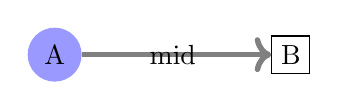
\begin{tikzpicture}
    \node[shape=circle, fill=blue!40] (node0) at ({0}, {0}) {A};
    \node[shape=rectangle, draw=black] (node1) at ({3}, {0}) {B};
    \draw[->, color=gray, line width=2] (node0) to (node1);
    \node (node2) at ({1.5}, {0.0}) {mid};
\end{tikzpicture}

\end{document}
